
In this chapter some basic theoretical insights about the BCDI technique are provided, with the aim to highlight the key 
concepts, assumptions and physical interpretations. More thorough descriptions can be found in papers, textbooks 
and PhD manuscripts. I will adopt the formalism of Als-Nielsen and McMorrow in \cite{alsnielsen_mcmorrow2011} but similar 
derivations and complementing observations can be found in \cite{guinier1994, paganin2006coherent} as well as some more recent papers \cite{vartanyants2013coherentxraydiffractionimaging} 
and PhD thesis \cite{dupraz:tel-01285735, girard:tel-02906931, Atlan2023}. 

\section{Foreword on typical assumptions and approximations in BCDI}
In order to keep the dissertation short and targeted to the BCDI case, I will start considering some observations on this
technique that will lead to some preliminary assumptions and simplifications. First, the word \textit{``Bragg''} suggests that 
crystalline specimens are involved. As discussed later in the text, Bragg's law applies to periodic structures, therefore 
we will limit our discussion to this specific case. \\
The word \textit{``Coherent''} implies that samples are probed with coherent beams (in our case X-rays). This fundamental property of 
electromagnetic radiation will be briefly discussed later on. For the moment, this ingredient enables us to approximate the 
probing radiation with plane electromagnetic waves. \\
The word \textit{``Diffraction''} refers to the type of mechanism describing the interaction between the X-rays and the 
samples. Paraphrasing \cite{guinier1994} at page 4, this mechanism can be divided into two main phenomena, namely (i) 
the scattering of the radiation by each individual atom in the sample and (ii) the interference between the waves scattered 
by these atoms. The interference mechanism, in turn, is enabled because these scattered waves are coherent with the incident 
radiation and therefore between themselves. In other words, the information of each scatterer is shared with the other scatterers 
as the diffracted waves ``talk to each other''. The complete mathematical description of these two phenomena without approximations 
is prohibitive, hence some simplifications usually adopted: 
\begin{itemize}
    \item \textbf{No refraction, no absorption}: Scattering is the only mechanism considered. Because of their short wavelengths
    (0.5 - 2.5 \AA), X-rays are practically never deviated by refraction. Moreover, we assume the absence of any absorption effect. 
    While inherently present, it can be neglected form small enough samples. 
    \item \textbf{Elastic scattering}: The interaction between the incoming X-rays and the atom is considered only elastic, meaning that 
    no energy is transferred to the atom, which bounces off instead the photons with unaltered energy and 
    momentum. This is again necessary for the scattered waves to interfere, as any difference in wavelength would 
    prevent any coherent interaction. This description, also called Thomson scattering, considers the interaction with a free charge, 
    and it also shows that cross-section of the scattering of electrons is much higher than the one of protons ($\sim 3\times10^{6}$ larger ). 
    For this reason, only the scattering from electrons is considered. 
    \item \textbf{Weak diffraction (Born approximation)}: This assumption implies that each scattered wave does not interact 
    further with the sample, therefore neglecting any possible multiple scattering event. The consequence of this assumption 
    is that the overall diffracted wave can be approximated by the linear superposition of the contributions of each scattering site. 
    This approximation, in crystallography, is called \textit{kinematical approximation}. 
    Dealing with crystalline samples, this assumption breaks for relatively thick samples ( $ > 1 \mu m $) in which the 
    light travels through the sample for longer distances before exiting, therefore bouncing off several atoms. 
    Diffraction of larger samples requires more complex theory of the so-called \textit{dynamical regime} \cite{takagi1969dynamical, gorobtsov2016phase, Shabalin2017}.
    However, in our case, the size of the typical samples studied with BCDI hardly exceeds $ 1 \mu m $ size, making the 
    kinematical approximation suitable. 
    % \item \textbf{Projection approximation}: According to Paganin \cite{paganin2006coherent}
    \item \textbf{Far-field approximation}: Here, the distance between the scattering atoms and the detector is assumed 
    to be much larger than the distance among the scatterers themselves. One can intuitively see that this approximation 
    turns the spherical waves created by the scatterers, interfering with each other, into plane waves when these are evaluated 
    far from the sources (in this case the sample's atoms). This assumption is always respected in the BCDI 
    technique as the sample-detector distance is in the order of tens of centimeters (practically from 30 cm to 2 m).

    % \item \textbf{Linear Polarization}: While not usual in textbooks, here, for simplicity we will consider linearly 
    % polarized x-rays. This restriction 

\end{itemize}

The last word \textit{``Imaging''} tells us that the format of the data is by nature, multidimensional (2D - 3D). It 
will be shown later in the chapter that 3D diffracted signal is recorded stacking 2D images captured by the detector, 
and therefore the results after the data analysis are 3D images of the sample.

Given this set of assumptions and approximations we can proceed with our simplified derivation of the equation governing 
the coherent X-ray scattering from a crystal and its interpretation. 

\section{Coherent X-ray scattering from crystalline structures}

Let us consider an X-ray beam, represented by a perfectly monochromatic plane wave with linear polarization in the horizontal 
plane, scattering with a single free electron (see Fig. \ref{fig:scattering}). In this simple case we can imagine the 
X-ray electromagnetic field exerting a force onto the electron placed at the origin of the reference frame. In turn, 
this force will accelerate the electron accordingly, therefore inducing an oscillation motion generating
an electromagnetic wave. Being the scattering assumed to be elastic, the radiation 
produced by the oscillating electron (\textit{electric dipole approximation}) will have the same wave-vector as the incoming X-ray. 
Moreover, the solution of Maxwell equations for this specific case 
shows that this dipole radiation propagates in the form of a spherical wave. At this point we ask ourselves what is the amplitude 
of this scattered wave when evaluated in a generic point $\mathbf r$ on the vertical plane, far from the origin (\textit{far-field approximation}). 
The result was achieved by Thomson in 1906 and is here reported without the full detailed derivation which can be found in the 
cited textbooks \cite{alsnielsen_mcmorrow2011,ashcroft_mermin1976, guinier1994}. 

% \begin{equation}
%     \mathbf{E}_{\text{dip}}(\mathbf{r},t) 
%     = r_e \, \frac{e^{ikr}}{r} \, e^{-i \omega t} 
%     \left[ \hat{r} \times \left( \hat{r} \times \mathbf{E}_0 \right) \right] 
%     e^{-i \mathbf{Q} \cdot \mathbf{r}'} 
%     \label{eq:scattering_pointlike}
% \end{equation}

\begin{equation}
    \mathbf{E}_{\text{dip}}(\mathbf{r},t) 
    = -r_0 \, \frac{e^{ikr}}{r} \, e^{-i \omega t} 
    E_0 \mathbf{\hat{z}}
    \label{eq:scattering_pointlike}
\end{equation}

where $r_0$ is the classical radius of the electron, or Thomson scattering length, $k$ is the outgoing wave-vector, $\omega$ is the pulsation of the 
X-ray beam (incoming and outgoing), $\mathbf{E}_0$ is the electric field of the incoming radiation.

In this case we cannot talk about diffraction as there is no interference of the outgoing wave with other scattered waves. In order 
to have a diffraction pattern we need to have at least a second charge scattering, from which a phase 
delay with respect to the first one can be calculated. For instance, if we consider $N$ electrons being illuminated by the 
same radiation, each of them placed in $\mathbf{r'}_n$ we could evaluate the contribution to the overall scattering 
wave-field for each electron. 
The simplest way is to make use of the \textit{kinematical approximation} and sum linearly all the contributions. However, we must 
take into account the phase delays between the scattering from different positions in space. 
This phase delay can be calculated, and it turns out to be $\Delta\phi(r) = (\mathbf k - \mathbf {k}_0)\cdot \mathbf{r}' = \mathbf Q \cdot \mathbf{r}'$ 
where we have expressed the difference between the wave vectors with $\mathbf{Q}$ often called \textit{scattering vector}.
The equation can thus be rewritten like: 

\begin{equation}
    \mathbf{E}_{\text{atom}}(\mathbf{r},t) 
    = r_e \, \frac{e^{ikr}}{r} \, e^{-i \omega t} 
    E_0 \mathbf{\hat{z}}
    \sum_{n = 1}^{N} e^{i \mathbf{Q} \cdot \mathbf{r}_n'} 
    \label{eq:scattering_electrons}
\end{equation}

In the continuum limit, replacing the $N$ point-like charges with an overall electron density distribution $\rho(\mathbf r)$ 
the above equation takes the form: 

\begin{equation}
    \mathbf{E}_{\text{atom}}(\mathbf{r},t) 
    = r_e \, \frac{e^{ikr}}{r} \, e^{-i \omega t} 
    E_0 \mathbf{\hat{z}}
    \int_{\mathbb{R}^3} \rho_a(\mathbf r') e^{i \mathbf{Q} \cdot \mathbf{r}'}  d^3 \mathbf r'
    \label{eq:scattering_atom}
\end{equation}

\begin{figure}[H]
    \centering
    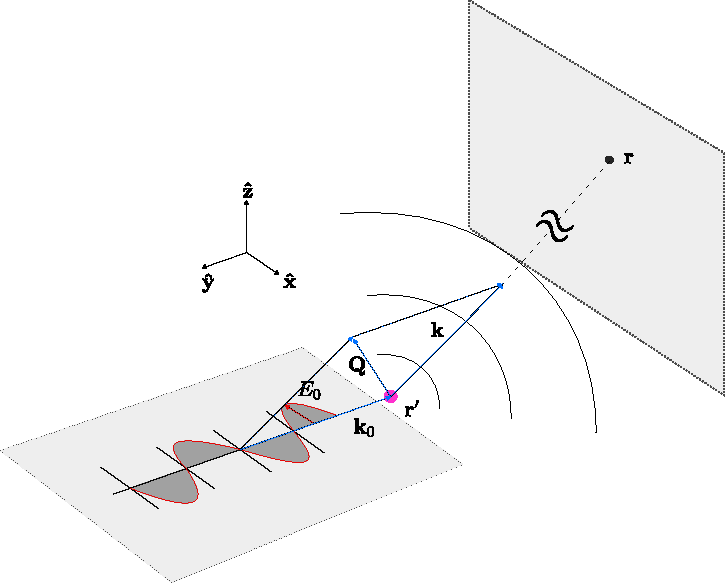
\includegraphics[width=\textwidth]{figures/Intro/scattering.pdf}
    \caption{Sketch of the scattering process evaluated in the far-field on the vertical plane for an electron density irradiated by a monochromatic X-ray beam 
    with linear polarization along the $\mathbf{\hat{x}}$ direction.}
    \label{fig:scattering}
\end{figure}

It is clear now that the information regarding the physical system of interest is embedded in the integral term. 
In fact, this is often called \textit{``form factor''} - $F(\mathbf Q)$ - and it plays an important role in the interpretation of the 
scattering equations. 

\begin{equation}
     F(\mathbf Q) = 
    \int_{\mathbb{R}^3} \rho(\mathbf r') e^{i \mathbf{Q} \cdot \mathbf{r}'}  d^3 \mathbf r'
    \label{eq:formfactor}
\end{equation}

$F(\mathbf{Q})$ represents the Fourier transform of the electron density, and it is the main result of this paragraph as it 
links the charge distribution of the sample in real space with the quantity measured, in reciprocal space. 

To continue, we should bear in mind that X-ray photon counting detectors are sensitive to the time-averaged intensity 
of the signal as their time response is much slower than the oscillating frequency of X-rays ($\sim 10^{9}$ Hz for typical 
read-out limited frame rates of the Maxipix 
\cite{ponchut_maxipix_2011} against the $\sim 10^{18}$ Hz for X-rays at 10 keV). This limitation is also at the core of 
the ``Phase Problem'' that we will see later on, for which the phase information of the complex-valued wave-field is 
lost in the measurement. 
In order to do so, the time-averaged Poynting vector is calculated. 

\begin{equation}
    \langle \mathbf{S(r)} \rangle = r_e^2 \frac{1}{r^2}J_0
    \left| \int \rho(\mathbf{r'}) e^{i \mathbf{Q}\cdot \mathbf{r'}} d^3 r' \right|^2 \mathbf{\hat{r}}
    \label{eq:poynting}
\end{equation}

where $J_0 = \left| \mathbf{E}_0 \right|^2 / 2\mu_0c$ is the incident intensity. 
To conclude we consider the power delivered on the detector. For a pixel with area $d\mathbf a = r^2d\Omega\mathbf{\hat{r}}$ 
the radiation power is equal to: 

\begin{equation}
    P(\mathbf{Q})= r_e^2 J_0
    \left| \int \rho(\mathbf{r'}) e^{i \mathbf{Q}\cdot \mathbf{r'}} d^3 r' \right|^2 d\Omega
    \label{eq:power}
\end{equation}

Eq.\ref{eq:power} shows that the signal captured by the detectors is now in $\mathbf{Q}$ space, and it is proportional 
to the square modulus of the Fourier transform of the electron density of the sample. The square modulus operation also 
shows how the phase of the Fourier transformed scattering complex-amplitude is lost. For this reason, in order to reconstruct 
the electron density, it is not possible to simply use an inverse Fourier transform, but iterative methods are required. 

\subsection{One atom}

If now we were to consider an atom, far from resonance, we could assume the electron density being the main responsible 
for the scattering. It is known indeed that protons, because of the larger mass, have a much smaller cross-section for the
scattering with photons. 
Using Eq.\ref{eq:formfactor} we would therefore have the \textit{atomic form factor} - $f_l(\mathbf{Q})$ being defined as: 

\begin{equation}
    f_l(\mathbf{Q}) = 
   \int_{\mathbb{R}^3} \rho_l(\mathbf r) e^{i \mathbf{Q} \cdot \mathbf{r}}  d^3 \mathbf r
   \label{eq:atomformfactor}
\end{equation} 

We now need to study the specific case in which the collection of atoms is ordered into a periodic structure. 

\subsection{Ensemble of ordered atoms: a Crystal}

Perfect crystals are constructed by a basic structural arrangement of atoms (\textit{motif}) repeated periodically on a 
\textit{lattice} of one or more dimensions. The regularity of the lattice is such that, for the 3D case, any of its nodes 
can be located in space by the formula: 

\begin{equation}
   \mathbf {R_n} = n_1\mathbf{a_1} + n_2\mathbf{a_2} + n_3\mathbf{a_3}
   \label{eq:lattice}
\end{equation}

where ${\mathbf{a_1},\mathbf{a_2},\mathbf{a_3}}$ constitutes the basis vectors of the primitive unit cell and $n_1, n_2, n_3$ are integer numbers. 
It follows that the information can be condensed in the unit cell, i.e. the orientation in space of the basis vectors as any region 
of the lattice can be seen as the same unit cell, translated from the origin by the amount given by $\mathbf {R_n}$. \\

The overall crystal is then constructed positioning on each of the nodes of the lattice the same motif, or basis. 

In another more elegant way, we could say that, being the lattice $\mathcal{L}(\mathbf r)$, the basis $\mathcal{B}(\mathbf r)$, the crystal 
$\mathcal{C}(\mathbf r)$ is given by the convolution of $\mathcal{L}(\mathbf r)$ with $\mathcal{B}(\mathbf r)$ : 

\begin{equation}
    \mathcal{C}(\mathbf r)  = \mathcal{L}(\mathbf r) \ast  \mathcal{B}(\mathbf r)  
    \label{eq:conv}
 \end{equation}

 For simplicity, we will consider from now on a single atom basis.
 At this point, when evaluating the scattering amplitude of the crystal we have to deal to an assembly of atoms, and we 
 may want to exploit the regular structure we have just described. 
 First, we can assume that, similarly to the case of many scattering electrons, in the kinematical approximation the overall 
 scattering factor is given by the sum of the contributions of each atom, weighted by a phase factor that accounts for their 
 positions in space. 

 \begin{equation}
    F_{\text{crystal}}(\mathbf{Q}) = 
   \sum_{l=1}^{\text{All atoms}} f_l(\mathbf Q) e^{i \mathbf{Q} \cdot \mathbf{r_l}} 
   \label{eq:crystalformfactor}
\end{equation} 

Secondly, observing that the position of each atom is given by the sum of the position of the atom inside the unit cell 
and the lattice vector $\mathbf{r_l} = \mathbf{R_n} + \mathbf{r_j}$, we can separate Eq.\ref{eq:crystalformfactor} in two terms: 

\begin{equation}
    F_{\text{crystal}}(\mathbf{Q}) = 
   \sum_{\mathbf{R_n} + \mathbf{r_j}}^{\text{All atoms}} f_l(\mathbf Q) e^{i \mathbf{Q} \cdot (\mathbf{R_n} + \mathbf{r_j})} = 
    \underbrace{\sum_{n} e^{i \mathbf{Q} \cdot \mathbf{R}_n}}_{\text{Lattice}}
    \underbrace{\sum_{j} f_j(\mathbf{Q}) e^{i \mathbf{Q} \cdot \mathbf{r}_j}}_{\text{Unit cell}}
   \label{eq:crystalformfactor2}
\end{equation} 

The first summation extends over all lattice points, while the second covers all atoms within the unit cell. 
Here we can already wrap the second sum into a more practical term expressing the \textit{unit cell form factor} 

\begin{equation}
    F_{\text{crystal}}(\mathbf{Q}) =  F_{\text{u.c}}(\mathbf{Q}) \sum_{n} e^{i \mathbf{Q} \cdot \mathbf{R}_n}
   \label{eq:crystalformfactor3}
\end{equation}

The term $ F_{\text{u.c}}(\mathbf{Q}) $ can be easily calculated as typical unit cells contain a small number of elements.
On the contrary we need to exploit the properties of the lattice periodicity to evaluate the large summation over all lattice 
points. 


\subsection{Laue condition and Bragg's Law} 

The term we want to calculate is the sum of complex exponential, meaning that if the phases $\mathbf{Q} \cdot \mathbf{R}_n$ 
are misaligned the sum will be \textit{incoherent} and the resultant will be very small, in the order of unity. 
On the contrary, when phase offsets are equal to an integer multiple of $2\pi$ the \textit{phasors} will add \textit{coherently} 
The problem is thus to find those $\mathbf{Q}$ values for which

\begin{equation}
   \mathbf{Q} \cdot \mathbf{R}_n = 2\pi \times \text{integer}  \qquad \forall n
   \label{eq:laue}
\end{equation}

In order to do than we need to construct a reciprocal space lattice with a set of basis ${\mathbf{a_1^\ast}, \mathbf{a_2^\ast}, \mathbf{a_3^\ast}}$ 
which fulfill: 

\begin{equation}
    \mathbf{a_1} \cdot \mathbf{a_1^\ast} = 2\pi h \qquad \mathbf{a_2} \cdot \mathbf{a_2^\ast} = 2\pi k \qquad \mathbf{a_3} \cdot \mathbf{a_3^\ast} = 2\pi l 
   \label{eq:miller}
\end{equation}

where $ h, k, l $ known as Miller indices, are integer. Having a set of basis vectors and the Miller indices, the 
resulting reciprocal space lattice lies in those points found by the vector $\mathbf{G}_{hkl}$ 

\begin{equation}
    \mathbf{G}_{hkl} =  h\mathbf{a_1^\ast} + k\mathbf{a_2^\ast} + l\mathbf{a_3^\ast} 
   \label{eq:G}
\end{equation}

This result is telling us that the scattering amplitude of a diffracting crystal is detectable only in those points of 
in space for which the wave-vector $\mathbf{Q}$ coincides with a point ($\mathbf{hkl}$ node) of the reciprocal lattice, 
hence $\mathbf{Q} = \mathbf{G}_{hkl}$. These isolated points are called \textit{Bragg peaks}.

This is known as the Laue condition for diffraction as it was discovered by Max von Laue in 1912 \cite{FriedrichKnippingLaue1912}.\\ 

A different but equivalent interpretation of the diffraction of a crystal was given by William Lawrence Bragg in 1913 \cite{Bragg1913}. 
Here, the crystal lattice is seen as a stack of parallel planes (see Fig.\ref{fig:bragg}) and the condition for constructive interference of 
the waves scattered by planes of the same family is found as follows.
Let us consider an X-ray beam of wavelength $\lambda$ and propagation vector $\mathbf{k_i} $ impinging with an angle $\theta$ 
on a crystal. We call $d_{hkl}$ the distance between the planes of the crystal, along a specific ${hkl}$ direction. The scattered 
beam is leaving the crystal with the 
same angle $\theta$ and with a propagation vector $\mathbf{k_f}$ equal in magnitude to the incident one (\textit{elastic scattering}). 
At this point one can find the relationship between $ \theta, d_{hkl}, \lambda$ that allows for a constructive interference of the 
waves diffracted from the series of planes by evaluating the optical path length difference induced by the spacing. 
Reminding that $\left|k_i\right| = \left|k_f\right| = 2\pi/\lambda $ and with the help of Fig. \ref{fig:bragg} we can observe that this 
difference is $\Delta l = 2 d_{hkl} \sin(\theta)$ and therefore the phase offset between two waves is $\Delta \phi = \left|k\right| \Delta l 
= 4 d_{hkl}\pi \sin(\theta)/\lambda $. We have seen above that the condition for constructive interference requires the phase 
differences to be equal to a multiple of $2\pi$, therefore: 

\begin{equation}
    2 d_{hkl} \sin(\theta) = n \lambda  \qquad \text{where  } n \in \mathbb{Z}
   \label{eq:Bragg}
\end{equation}

Moreover, it can be shown that the family of planes is defined by the vector $G_{hkl}$ which points at the reciprocal space 
node that is collecting the scattering from those planes, and defines as well the spacing $d_{hkl}$ between each of 
these planes. 

\begin{figure}[H]
    \centering
    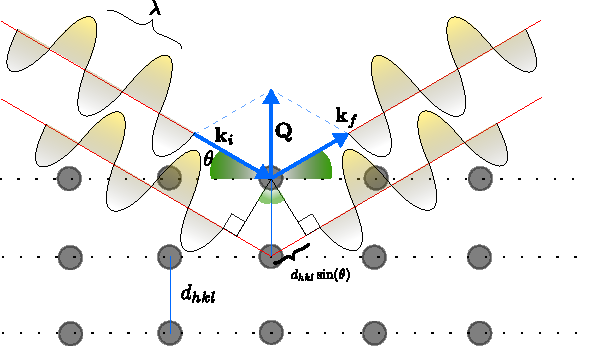
\includegraphics[width=\textwidth]{figures/Intro/bragg.pdf}
    \caption{Illustration of Bragg's law. The family of crystal planes given separated by $d_{hkl}$ produces constructive interference 
    when the incident radiation illuminates it with an angle  $\theta$ given by Eq.\ref{eq:Bragg}.} 
    \label{fig:bragg}
\end{figure}

Equation \ref{eq:Bragg} is known as Bragg's law, and it can be derived from the Laue condition. 

We can now rewrite Eq.\ref{eq:crystalformfactor3} for the case of an infinitely extended perfect 3D crystal as: 

\begin{equation}
    F_{\text{crystal}^{\infty}}(\mathbf{Q}) = F_{\text{u.c.}}(\mathbf{Q}) 
    \sum_{h} \sum_{k} \sum_{l} 
    \delta\!\left(\mathbf Q - \mathbf{G}_{hkl}\right)
    \label{eq:crystalformfactor4}
\end{equation}
    
where the term relative to the lattice is expressed as the sum of Dirac deltas in $Q$ space centered in each $hkl$ node. 


\subsection{Finite size crystals}

We are now ready to treat the case of finite size crystals. In the above description the lattice was assumed to extend 
infinitely along all the 3 dimensions. This, we have seen, results in a scattering signal that lives on a perfect reciprocal 
lattice made of point-like nodes. Because of the Fourier transformation that links the real space scattering object and 
the reciprocal space diffracted signal, one can intuitively deduce that if for an infinite crystal we obtain a point-like 
Bragg peaks, we could expect a broadening of the peaks as the crystal size is reduced. 

Mathematically we can derive the result for crystal of shape $S(\mathbf r)$ considering the function $S$ a window cropping 
a finite portion of the 3D infinite crystal. This function can also be referred to as Ewald function \cite{Ewald_1940} or \textit{support}.
 In real space this corresponds to the product: 


\begin{equation}
    \rho_{\text{fin}}(\mathbf{r}) = \rho_{\infty}(\mathbf{r}) S(\mathbf{r})
    \label{eq:window}
\end{equation}

where 

\begin{equation}
    S(\mathbf r) \;=\;
    \begin{cases}
    1, & \text{inside the crystal region}
    , \\[6pt]
    0, & \text{otherwise}.
    \end{cases}
    \label{eq:shape_function_general}
\end{equation}
    
For the convolution theorem we have now that the Fourier transform $\mathcal{F\{}{\rho_{\text{fin}}(\mathbf{r})\}}$ is 
equal to the convolution $ \mathcal{F\{}{\rho_{\infty}(\mathbf{r})\} \ast \mathcal{F\{}S(\mathbf{r})\}}$. 
Using Eq.\ref{eq:crystalformfactor3} for the Fourier transform of the infinite crystal and calling $\widehat S(\mathbf{Q})= \mathcal{F} \{S(\mathbf{r})\}$ 
we can therefore write: 

\begin{equation}
    F_{\text{fin. crystal}}(\mathbf{Q}) = \Big[ F_{\text{u.c.}}(\mathbf{Q}) 
    \sum_{h} \sum_{k} \sum_{l} 
    \delta\!\left(\mathbf Q - \mathbf{G}_{hkl}\right) \Big] \ast \widehat S(\mathbf{Q})
    \label{eq:fin_cryst1}
\end{equation}

For the commutative property of convolutions, we can now rearrange the terms as follows: 

% \begin{equation}
%     F_{\text{fin. crystal}}(\mathbf{Q}) = \sum_{h} \sum_{k} \sum_{l} (F_{\text{u.c.}}\ast \widehat S)
%     (\mathbf{Q} - \mathbf{G}_{hkl}) = \sum_{h} \sum_{k} \sum_{l} \int F_{\text{u.c.}}(\mathbf{Q'})\widehat S
%     (\mathbf{Q} - \mathbf{G}_{hkl} -\mathbf{Q'}) d^3\mathbf{Q'}
%     \label{eq:fin_cryst2}
% \end{equation}

\begin{equation}
    \begin{aligned}
    F_{\text{fin. crystal}}(\mathbf{Q}) &= 
    \widehat S(\mathbf{Q}) \ast  \Big[ F_{\text{u.c.}}(\mathbf{Q}) \sum_{h} \sum_{k} \sum_{l} \delta\!\left(\mathbf Q - \mathbf{G}_{hkl}\right) \Big] \\
    &= \int \widehat S(\mathbf{Q} -\mathbf{Q'}) F_{\text{u.c.}}(\mathbf{Q'}) \sum_{h} \sum_{k} \sum_{l} \delta\!\left(\mathbf Q' - \mathbf{G}_{hkl}\right) d^3\mathbf{Q'} 
    \end{aligned} 
    \label{eq:fin_cryst2}
\end{equation}

At this point, we can bring the integral inside the summation and calculate: 

\begin{equation}
    \begin{aligned}
    F_{\text{fin. crystal}}(\mathbf{Q}) &= 
    \sum_{h} \sum_{k} \sum_{l} \int \widehat S(\mathbf{Q} -\mathbf{Q'}) F_{\text{u.c.}}(\mathbf{Q'}) \delta\!\left(\mathbf Q' - \mathbf{G}_{hkl}\right) d^3\mathbf{Q'} 
    \end{aligned} 
    \label{eq:fin_cryst3}
\end{equation}

We observe now that the Dirac delta function is non-zero only in the $hkl$ nodes defined by $\mathbf{G}_{hkl}$. 
This leads to the final equation: 
% in order to evaluate the convolution integral in Eq. \ref{eq:fin_cryst2} we can assume the unit cell 
% to be much smaller than the crystal support. This is typically the case in BCDI. This assumption allows us to consider 
% the Fourier transform of the unit cell $F_{\text{u.c.}}$ to be slowly varying (i.e. ``constant'') with respect to the 
% Fourier transform of the crystal. Moreover, assuming the crystal to contain a large number of unit cells, means condensing 
% most of the scattering signal around the $\mathbf Q = \mathbf{G}_{hkl}$, thus  $\mathbf {Q'} = \mathbf{0}$. We can therefore rewrite: 

\begin{equation}
    F_{\text{finite}}(\mathbf{Q}) = 
    \sum_{h} \sum_{k} \sum_{l} \widehat S(\mathbf Q - \mathbf{G}_{hkl})F_{\text{u.c.}}(\mathbf{G}_{hkl})
    \label{eq:fin_cryst3}
\end{equation}

Here we see that the Bragg peaks, from point-like spots in reciprocal space are subjected to a broadening that shapes them 
according to the structure of the Fourier transform of the crystal shape, centered at $\mathbf{G}_{hkl}$. \\

Let us now consider the specific case of a cubic crystal aligned with the direct-lattice basis $\mathbf{a_1},\mathbf{a_2},\mathbf{a_3}$.
The crystal contains $N$ cells along each basis vector $\mathbf{a}$. Each edge vector is therefore $\mathbf{L}_j = N\mathbf{a}_j$ 
Being the center of the cubic crystal placed in the origin of the reference frame we can now write the support function as: 

\begin{equation}
    S(\mathbf r) \;=\; 
    \prod_{j=1}^{3} \mathcal R \,\!\left(\frac{\mathbf{r} \cdot \mathbf{\hat{a}}_j}{L_j}\right),
    \qquad
    \mathcal R(x) \;=\;
    \begin{cases}
    1, & |x| \le 1/2
    , \\[6pt]
    0, & \text{else}.
    \end{cases}
    \label{eq:cube}
\end{equation}

where $\mathbf{\hat{a}}_j = \mathbf{a}_j/|\mathbf{a}_j|$ and $L_j = \mathbf{L}_j/|\mathbf{L}_j|$, and the 1D rectangular function
$ \mathcal R(x)$ has been defined. Here we have defined the cube as the product of the three 1D rectangular function on each 
of the 3 dimensions. We can therefore calculate the Fourier transform of $S(\mathbf{r})$ as the product of the Fourier 
transform of each $\mathcal{R}\left(\frac{\mathbf{r} \cdot \mathbf{\hat{a}}_j}{L_j}\right)$. 

It follows that: 

\begin{equation}
    \widehat S(\mathbf Q) \;=\; 
    \prod_{j=1}^{3} L_j \,\!\operatorname{sinc}\left(\frac{\mathbf{Q} \cdot \mathbf{\hat{a}}_j L_j}{2}\right),
\end{equation}

where we made use of the cardinal sine function defined as $\operatorname{sinc}(x) = \frac{\sin x}{x}$. 
Putting this result in Eq. \ref{eq:fin_cryst3} we obtain: 

\begin{equation}
    F_{\text{cube}}(\mathbf Q) \;=\; 
    \sum_{h} \sum_{k} \sum_{l} F_{\text{u.c.}}(\mathbf{G}_{hkl})\,
    \prod_{j=1}^{3} L_j \,\!\operatorname{sinc}\left(\frac{(\mathbf{Q}- \mathbf{G}_{hkl}) \cdot \mathbf{\hat{a}}_j L_j}{2}\right),
    \label{eq:cube_bragg}
\end{equation}

At this point of the derivation we can introduce another simplification, directly linked to the BCDI technique.
Up to now we have been considering the scattering amplitude in the full reciprocal space. This means that Eq. \ref{eq:cube_bragg}
is encompassing all the $hkl$ nodes in which we could find the diffracted signal. However, in typical BCDI experiments 
only a small region around a single Bragg peak is measured. This means that we can from now on focus on one $\mathbf{G}_{hkl}$ 
vector and drop the summation.  Moreover, defining $\mathbf q = \mathbf{Q}- \mathbf{G}_{hkl}$ and recalling the result obtained in Eq.\ref{eq:power} 
one can find that the intensity of the diffraction pattern of the $hkl$ Bragg peak is : 

\begin{equation}
    I_{\text{cube}}(\mathbf q) \;\propto\; 
    F_{\text{u.c.}}(\mathbf{G}_{hkl})\,
    \left | \prod_{j=1}^{3} L_j \,\!\operatorname{sinc}\left(\frac{\mathbf{q} \cdot \mathbf{\hat{a}}_j L_j}{2}\right)\right|^2,
    \label{eq:cube_bragg2}
\end{equation}

The diffracted signal for a cubic crystal in the vicinity of the $hkl$ Bragg peak has therefore 
the shape of a \textit{squared} 3D cardinal sine function as represented in Fig. \ref{fig:cube}

\begin{figure}[H]
    \centering
    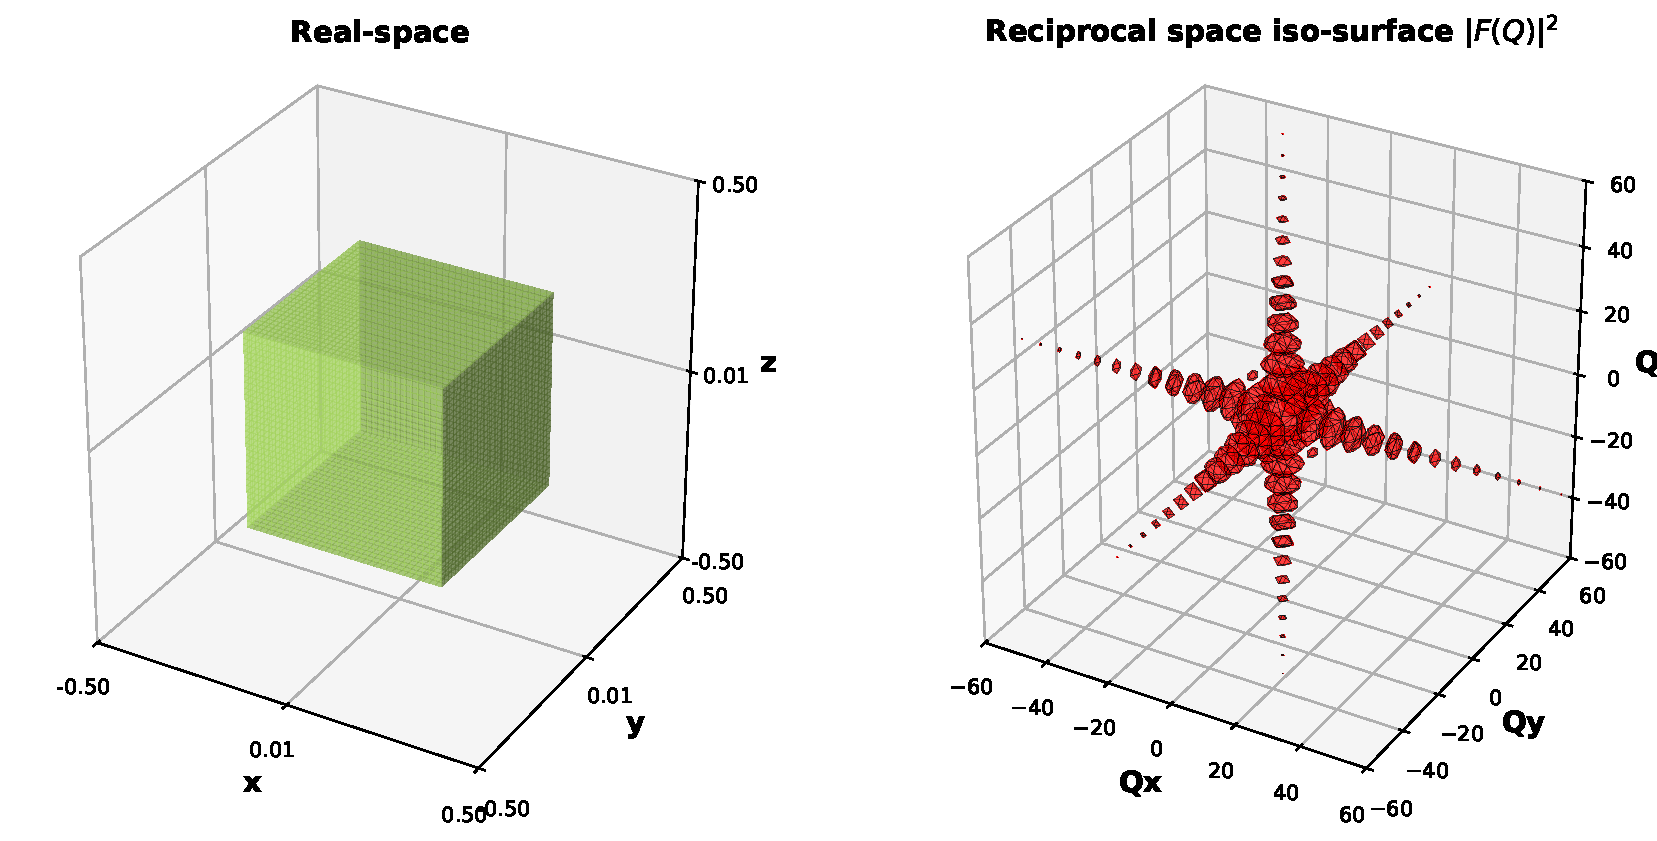
\includegraphics[width=\textwidth]{figures/Intro/cube1.pdf}
    \caption{Illustration of the squared modulus of the Fourier transform of cube as representation of the diffracted 
    intensity around a Bragg peak for a cubic crystal. }
    \label{fig:cube}
\end{figure}

An interesting observation concerns the spacing between the fringes of the interference pattern. Studying Eq.\ref{eq:cube_bragg2}
we can infer that:  

\begin{itemize}
    \item The maximum of the peak is concentrated at $\mathbf q = 0  \Rightarrow \mathbf Q = \mathbf{G}_{hkl}$ as expected. 
    \item The intensity decays as $ \sim 1/\mathbf{q}^2$ along the intensity streaks, also known as crystal truncation 
    rods (CTR) \cite{Robinson1986CTR}. This decay depends on the shape. For a spherical crystal it follows a $ \sim 1/\mathbf{q}^4$ law.
    \item The 
    intensity drops to zero every time the argument $(\mathbf{q} \cdot \mathbf{\hat{a}}_j L) /2 = n\pi$ with $n$ integer. 
    This results in the presence of fringes that have a thickness as a function of the $\mathbf q$ direction given by:
    $\Delta q_j = 2\pi/L$. 
    \item Given the above relationship between the thickness of the fringes and the size of the crystal, one can intuitively
    imagine extending $L$ to infinity, thus narrowing the fringes to zero width and the central lobe to a Dirac delta in $\mathbf{q} = 0$ 
    as in the infinite lattice case. 
\end{itemize}

\begin{figure}[H]
    \centering
    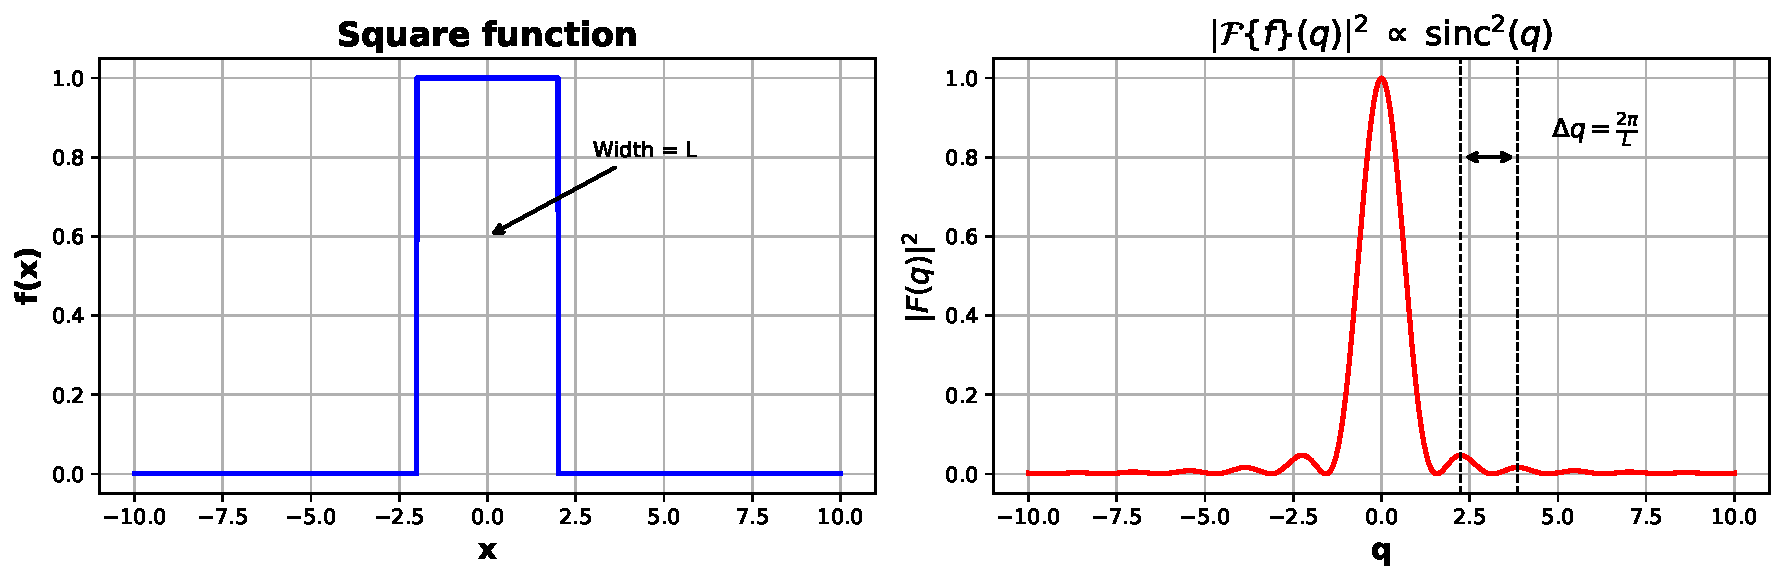
\includegraphics[width=\textwidth]{figures/Intro/square.pdf}
    \caption{1D example of the squared modulus of the Fourier transform of a square function. The sharp intensity decay 
     outside the central peak is evident. The spacing between fringes of constructive interferences is also related 
     to the width of the square.}
    \label{fig:square_ft}
\end{figure}

For the understanding and visualization of Fourier transforms in crystallography I recommend the pedagogical work of 
Aubert and Lecombte \cite{Aubert:kk5014}.

\subsection{Real crystals}
We are now ready to deal with non-perfect crystals. The presence of surfaces, substrates, physio-chemical reaction with 
the environment induce deformations of the perfect crystalline structure. In the most general case the deformation is 
modeled by a displacement field $\mathbf{u(r)}$ 
that shifts the position of each atom of the crystal off the position of the perfect lattice. However, for simplicity 
the displacement field is often assumed to act on the whole unit cell rather than each single atom. One can therefore 
write the scattering amplitude as the sum over the unit cells. 
Defining $\mathbf{u}(\mathbf{R}_n)$ the displacement of the $n-th$ cell with respect to the perfect lattice position 
we can calculate the structure factor of the infinite crystal summing over all the unit cells the form factor of each cell weighted by 
their displaced positions: 

\begin{equation}
    F^{\text{strain}}_{\infty}(\mathbf{Q}) = 
    \sum_{n} F_n(\mathbf{Q}) e^{i \mathbf{Q} \cdot (\mathbf{R}_n + \mathbf{u}(\mathbf{R}_n))}
   \label{eq:strain1}
\end{equation} 

To lighten up the notation we can introduce another vector $\mathbf{R}'_n = \mathbf{R}_n + \mathbf{u}(\mathbf{R}_n)$ that 
points at each displaced unit cell. Being this lattice no longer perfectly periodic we cannot any more simplify the sum 
into a sum of delta functions calculated in the $hkl$ nodes of the reciprocal lattice. 
At this point we can however repeat the calculations for the case of a finite size crystal of shape $S(\mathbf{r})$. 
For the convolution theorem we can write: 

\begin{equation}
    F^{\text{strain}}_{\text{fin}}(\mathbf{Q}) = 
    \sum_{n} F_n(\mathbf{Q}) e^{i \mathbf{Q} \cdot \mathbf{R}'_n} \ast \widehat{S}(\mathbf{Q})
   \label{eq:strain_fin}
\end{equation}

Developing the convolution integral we obtain: 

\begin{equation}
    \begin{aligned}
    F^{\text{strain}}_{\text{fin}}(\mathbf{Q}) &= 
    \int \sum_{n} F_n(\mathbf{Q} -\mathbf{Q'}) e^{i (\mathbf{Q}-\mathbf{Q'}) \cdot \mathbf{R}'_n} \widehat{S}(\mathbf{Q'})d^3\mathbf{Q'} \\
    &= \sum_{n} \int F_n(\mathbf{Q} -\mathbf{Q'}) e^{i (\mathbf{Q}-\mathbf{Q'}) \cdot \mathbf{R}'_n} \widehat{S}(\mathbf{Q'})d^3\mathbf{Q'} \\ 
   \label{eq:strain_fin2}
    \end{aligned}
\end{equation}

where, being the sum over a finite number of unit cells converging, we moved the integral sign inside the sum. 
Now, we can assume to restrict the field of view in the vicinity of the $\mathbf{G}_{hkl}$ where the unit cell 
form factor varies slowly compared to the $\widehat{S}(\mathbf{Q'})$. Intuitively we could understand this step considering 
that typical BCDI crystals contain a large number of unit cells, therefore in Fourier space, the features relative to 
the crystal shape vary much faster than the features relative to the unit cell. This approximation allows us to write:
% Now, similarly to Eq.\ref{eq:fin_cryst3}, we can bring the unit cell form factor outside the integral for crystals containing 
% a large number of unit cells.  
Hence: 

\begin{equation}
    \begin{aligned}
    F^{\text{strain}}_{\text{fin}}(\mathbf{Q}) &=  
    \sum_{n} F_n(\mathbf{G}_{hkl}) \int  e^{i (\mathbf{Q} -\mathbf{Q'}) \cdot \mathbf{R}'_n} \widehat{S}(\mathbf{Q'})d^3\mathbf{Q'} \\ 
    &= \sum_{n} F_n(\mathbf{G}_{hkl}) \int  e^{i \mathbf{Q} \cdot \mathbf{R}'_n } e^{-i \mathbf{Q'} \cdot \mathbf{R}'_n} \widehat{S}(\mathbf{Q'})d^3\mathbf{Q'} \\ 
    &= \sum_{n} F_n(\mathbf{G}_{hkl}) e^{i \mathbf{Q} \cdot \mathbf{R}'_n } \int e^{-i \mathbf{Q'} \cdot \mathbf{R}'_n} \widehat{S}(\mathbf{Q'})d^3\mathbf{Q'} \\ 
    &= \sum_{n} F_n(\mathbf{G}_{hkl}) e^{i \mathbf{Q} \cdot \mathbf{R}'_n } S(\mathbf{R}'_n) \\
   \label{eq:strain_fin3}
    \end{aligned}
\end{equation}

where we have recognized the inverse Fourier transform of the shape function calculated in $\mathbf{R}'_n$. 
If we now assume that the displacement affecting each unit cell does not influence the form factor, 
we can replace $F_n(\mathbf{G}_{hkl})$ with $F_{\text{u.c.}}(\mathbf{G}_{hkl})$ and take it out of the sum. 
Additionally, considering the relations $\mathbf{Q} = \mathbf{G}_{hkl} + \mathbf{q}$ and $e^{i \mathbf{G}_{hkl} \cdot \mathbf{R}_n}  = 1$
we can rearrange into: 

\begin{equation}
    \begin{aligned}
        F^{\text{strain}}_{\text{fin}}(\mathbf{Q}) &= 
        \sum_{n} F_n(\mathbf{G}_{hkl}) e^{i \mathbf{Q} \cdot \mathbf{R}'_n} S(\mathbf{R}'_n) \\
        &= F_{\text{u.c.}}(\mathbf{G}_{hkl}) \sum_{n}  e^{i (\mathbf{G}_{hkl} + \mathbf{q}) \cdot  (\mathbf{R}_n + \mathbf{u}(\mathbf{R}_n)) } S(\mathbf{R}'_n) \\
        &= F_{\text{u.c.}}(\mathbf{G}_{hkl}) \sum_{n}  e^{i \mathbf{G}_{hkl}\cdot  \mathbf{R}_n} e^{i \mathbf{G}_{hkl} \cdot  \mathbf{u}(\mathbf{R}_n) } e^{i \mathbf{q} \cdot  (\mathbf{R}_n + \mathbf{u}(\mathbf{R}_n)) } S(\mathbf{R}'_n) \\
        &= F_{\text{u.c.}}(\mathbf{G}_{hkl}) \sum_{n} S(\mathbf{R}'_n) e^{i \mathbf{G}_{hkl} \cdot  \mathbf{u}(\mathbf{R}_n) } e^{i \mathbf{q} \cdot  \mathbf{R}'_n }
    \end{aligned}
    \label{eq:strain_fin4}
\end{equation}

The formula we obtained tells us that scattering amplitude for the finite strained crystal is proportional to the 
sum over all the unit cells of the shape function evaluated in each displaced unit cell times a two phase factors. 
The first phase factor is given by the projection of the displacement of each unit cell (relative to the perfect lattice) 
onto the scattering vector of the given $hkl$ node. This term is relevant in BCDI experiments as it is directly linked to 
the strain and more general information on the internal lattice displacements of the particle. 
The second complex exponential evaluates the phase delay associated to each displaced unit cell with respect to the 
center of Bragg peak. 

Despite the close similarity to a classical discrete Fourier transform (DFT), one should notice that the variable $\mathbf{R}'_n)$ 
is not uniform as the displacements disrupt the regular periodicity of the grid, required for a standard Fourier transform. 
It is therefore common to approximate this non-uniform discrete Fourier transform with a standard discrete one by assuming: 

\begin{itemize}

    \item $\mathbf{q}\cdot\mathbf{u}(\mathbf{R}_n) = 0 $ which means that the projection of the displacements on the vector 
    $\mathbf{q}$ originating in the $hkl$ and exploring the vicinity of the Bragg peak, is small. Given the relatively 
    reduced volume of $\mathbf{q}$-space around the Bragg peak that is usually probed in BCDI this approximation is 
    also reasonable. This is also known as the Takagi approximation \cite{takagi1969dynamical}. When this approximation is applied Eq.\ref{eq:strain_fin4} takes the form of the so-called \textit{kinematic sum}
    and it is implemented in software for simulation of diffraction 
    patterns starting from atomic positions like, for instance, the \texttt{scattering} module of PyNX \cite{pynx_scattering}. 

    \item $ S(\mathbf{R}'_n) = S(\mathbf{R}_n)$, which means that the shape function is not altered by the internal or superficial 
    displacements. This is the case for displacements much smaller than the lattice parameter, which is easily fulfilled in 
    typical BCDI samples. In practice, this approximation allows to describe the electron density on a periodic grid. 
     
\end{itemize}

At this point, embedding the $e^{i \mathbf{G}_{hkl} \cdot  \mathbf{u}(\mathbf{R}_n) }$ in a more general \textit{complex-valued 
shape function} $\tilde{S}$ and considering now the intensity of the signal impinging on the detector, we can write: 

\begin{equation}
    F^{\text{strain}}_{\text{fin}}(\mathbf{q}) = F_{\text{u.c.}}(\mathbf{G}_{hkl}) \sum_{n} \tilde{S}(\mathbf{R}_n) e^{i \mathbf{q} \cdot  \mathbf{R}_n }
    \label{eq:strain_fin4}
\end{equation}

where we have now put the reference frame in the center of the Bragg peak at the $hkl$ position, therefore expressing 
the scattering factor as function of $\mathbf{q}$.
% We should now introduce a local momentum vector $\mathbf{q}$, defined in the vicinity of the $hkl$ node. 

% \begin{equation}
%    \mathbf{Q} = \mathbf{G}_{hkl} + \mathbf{q}
%    \label{eq:q}
% \end{equation} 

% Eq. \ref{eq:strain1} assumes the equivalent form: 

% \begin{equation}
%     F^{\text{strain}}_{\infty}(\mathbf{G}_{hkl} + \mathbf{q}) = 
%     F_{\text{u.c.}}(\mathbf{G}_{hkl} + \mathbf{q}) \sum_{n} e^{i (\mathbf{G}_{hkl} + \mathbf{q}) \cdot \mathbf{u}(\mathbf{R}_n)} e^{i \mathbf{Q} \cdot \mathbf{R}_n}
%    \label{eq:strain2}
% \end{equation} 

% At this stage we can make two approximations that will simplify the derivation. First, similarly to Eq.\ref{eq:cube_bragg2} where 
% we assumed the Fourier transform of the unit cell slowly varying, we can now repeat and obtain $F_{\text{u.c.}}(\mathbf{G}_{hkl} + \mathbf{q}) 
% = F_{\text{u.c.}}(\mathbf{G}_{hkl})$. 
% For the second approximation, let us remind that $\mathbf{G}_{hkl}$ points to a single fixed $hkl$ node and $\mathbf{p}$ is a vector departing from 
% the $hkl$ node and ``exploring'' its vicinity. We can therefore assume that for relatively small displacements the 
% contribution of the term $\mathbf{q}\cdot\mathbf{u}(\mathbf{R}_n)$ is much smaller than the term $\mathbf{G}_{hkl}\cdot\mathbf{u}(\mathbf{R}_n)$
% hence, negligible in first approximation. 
% Rearranging the terms, Eq.\ref{eq:strain2} takes now the form: 

% \begin{equation}
%     F^{\text{strain}}_{\infty}(\mathbf{G}_{hkl}) = 
%     F_{\text{u.c.}}(\mathbf{G}_{hkl}) \sum_{n} e^{i \mathbf{Q} \cdot \mathbf{R}_n} e^{i \mathbf{G}_{hkl} \cdot \mathbf{u}(\mathbf{R}_n)} 
%    \label{eq:strain3}
% \end{equation} 

% We can now recognize Eq.\ref{eq:crystalformfactor3} calculated in the $hkl$ node, with the addition of a phase term 
% accounting for the displacement of each unit cell in the lattice. At this point, we can move to the case of a finite size 
% crystal and, recalling Eq.\ref{eq:fin_cryst1}, we can write: 

% \begin{equation}
%     F^{\text{strain}}_{\text{finite}}(\mathbf{G}_{hkl}) = 
%     \big [ F_{\text{u.c.}}(\mathbf{G}_{hkl}) \sum_{n} e^{i \mathbf{Q} \cdot \mathbf{R}_n} e^{i \mathbf{G}_{hkl} \cdot \mathbf{u}(\mathbf{R}_n)} 
%     \big] \ast \widehat{S}(\mathbf{Q})
%    \label{eq:fin_strain1}
% \end{equation} 

% Writing the full convolution integral we obtain: 

% \begin{equation}
%     F^{\text{strain}}_{\text{finite}}(\mathbf{G}_{hkl}) = \int
%     F_{\text{u.c.}}(\mathbf{G}_{hkl}) \sum_{n} e^{i \mathbf{(Q - Q')} \cdot \mathbf{R}_n} e^{i \mathbf{G}_{hkl} \cdot \mathbf{u}(\mathbf{R}_n)} \widehat{S}(\mathbf{Q'})d^3\mathbf{Q'}
%    \label{eq:fin_strain2}
% \end{equation}

% Being the sum over the finite number of lattice points converging, we can bring the integral inside and rearrange. 
% \begin{equation}
%     F^{\text{strain}}_{\text{finite}}(\mathbf{G}_{hkl}) =
%     F_{\text{u.c.}}(\mathbf{G}_{hkl}) \sum_{n} e^{i \mathbf{G}_{hkl} \cdot \mathbf{u}(\mathbf{R}_n)} e^{i \mathbf{Q} \cdot \mathbf{R}_n} \int \widehat{S}(\mathbf{Q'}) e^{-i \mathbf{Q'} \cdot \mathbf{R}_n}d^3\mathbf{Q'}      
%    \label{eq:fin_strain3}
% \end{equation}

% At this point we should recognize the inverse Fourier transform of the $\widehat{S}(\mathbf{Q'})$ term evaluated in the direct 
% lattice point $\mathbf{R}_n$. 
% The equation therefore becomes: 

% \begin{equation}
%     \begin{aligned}
%     F^{\text{strain}}_{\text{finite}}(\mathbf{G}_{hkl}) =
%     F_{\text{u.c.}}(\mathbf{G}_{hkl}) \sum_{n} S(\mathbf{R}_n) e^{i \mathbf{G}_{hkl} \cdot \mathbf{u}(\mathbf{R}_n)} e^{i \mathbf{Q} \cdot \mathbf{R}_n}  \\
%     = F_{\text{u.c.}}(\mathbf{G}_{hkl}) \sum_{n} \tilde S (\mathbf{R}_n) e^{i \mathbf{Q} \cdot \mathbf{R}_n} \\
%     = F_{\text{u.c.}}(\mathbf{G}_{hkl}) \sum_{n} \tilde S (\mathbf{R}_n) e^{i \mathbf{G}_{hkl} \cdot \mathbf{R}_n} e^{i \mathbf{q} \cdot \mathbf{R}_n} \\ 
%     = F_{\text{u.c.}}(\mathbf{G}_{hkl}) \sum_{n} \tilde S (\mathbf{R}_n) e^{i \mathbf{q} \cdot \mathbf{R}_n}
%     \end{aligned}
%     \label{eq:fin_strain4}
% \end{equation}

% where we have used Eq.\ref{eq:q} and integrated the exponential term including the displacement field in a more general \textit{complex-valued shape function}. 
% Eq.\ref{eq:fin_strain4} contains the sum over all lattice nodes of the finite crystal of the complex-valued shape function 
% weighted by the complex exponential term accounting for the phase delay relative to each site, with respect to the considered 
% $hkl$ Bragg peak. In other words, 
% it represents the \textit{discrete} Fourier transform of $\tilde S (\mathbf{R}_n)$ considered in the vicinity of a given $\mathbf{G}_{hkl}$ vector. 
 

% Finally, we can write the scattering intensity as: 

% \begin{equation}
%     I^{\text{strain}}_{\text{finite}}(\mathbf q) \;\propto\; 
%     \left| F_{\text{u.c.}}(\mathbf{G}_{hkl}) \right|^2 
%     \left| \mathcal{F}\!\left\{ \tilde S(\mathbf{R}_n) \right\} \right|^2
%     \label{eq:strain_int}
% \end{equation}
Eq.\ref{eq:strain_fin4} is now a discrete Fourier transform (DFT) of $\tilde{S}(\mathbf{R}_n)$ calculated over the $n$ 
points in coordinates $R_n$ of the perfect crystal lattice and is the most important result of the chapter. 
Lastly, it is important to mention that when dealing with numerically computed DFT, in 3D, instead of the point-like 
$\mathbf{R}_n$ coordinate, a general coordinate $\mathbf{r}$ pointing at voxels of size $\delta r_i \sim 1/q^\text{max}_i$ 
(where $q^\text{max}_i$ is the extent of the Fourier window along the $i$-th dimension) is used. Moreover, later in the manuscript we will always refer to this complex-valued 
shape function as the ``\textit{complex object}'' or ``\textit{reconstructed particle}'' and will often deal with its 
complex phase. 

Specifically it will be used for simplicity the following relationship, which is derived like \ref{eq:power} and drops all the constant terms: 

\begin{equation}
    I(\mathbf q) =  \left| \mathcal{F}\!\left\{ \rho(\mathbf{r}) e^{i \phi(\mathbf{r})} \right\} \right |^2
    \label{eq:fourie_relation}
\end{equation}

Eq.\ref{eq:fourie_relation} has the advantage of expressing the diffraction pattern with a DFT, which allows for 
fast computations via efficient algorithms, rather than a sum evaluated in each individual unit cell position. This 
represents a key ingredient for the most used phase retrieval algorithms in BCDI (as we will see in the next Chapter), 
due to the large number of DFT operations required. Interesting works have evaluated the validity of these approximations
\cite{Godard2021} and the discrepancy between diffraction patterns calculated with the DFT and kinematic sum \cite{Haag2013, Madsen2021}
of 

\begin{figure}[H]
    \centering
    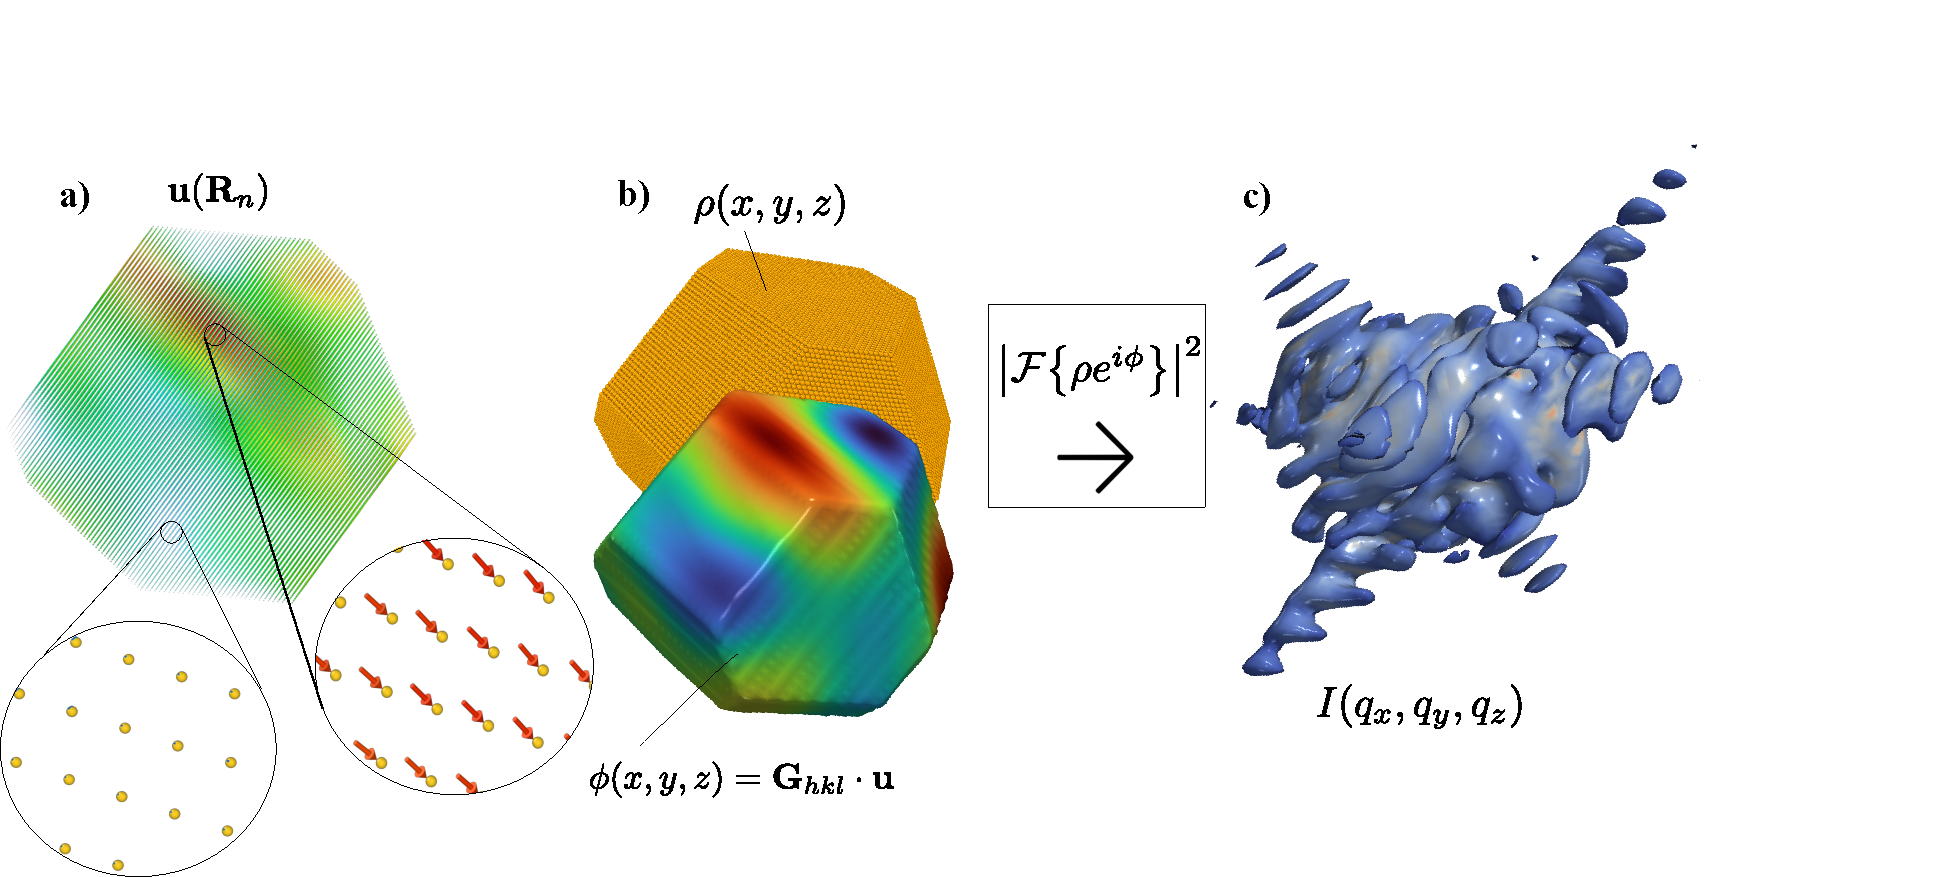
\includegraphics[width=\textwidth]{figures/Intro/displacement.pdf}
    \caption{Schematic of the relationship between displacement field and diffraction pattern. \textbf{a)} Simulated 
    displacement field obtained from the subtraction of the atomic positions of a simulated strained gold crystal with 
    the relative perfect lattice copy. Close-up on two different regions where the displacement is small (left) and large (right). 
    \textbf{b)} Formulation of the scattering object as a complex object. The modulus being interpreted as the electronic 
    density and the phase being the projection of the displacement on the scattering vector pointing at the probed $hkl$ node. 
    \textbf{c)} Corresponding diffraction pattern proportional to the square modulus of the Fourier transform of the complex object.}
    \label{fig:displacement}
\end{figure}

It is interesting here to analyze what the effect of the displacement is on the shape of diffraction pattern. Intuitively 
we can think that the complex phase term is altering the interference of the scattered waves. If, for a perfect lattice, we 
had Dirac deltas broadened and modulated by the Fourier transform of the shape function, here we have to consider an additional 
broadening due to the strain. Moreover, we know from Friedel's law \cite{Friedel} that the diffraction pattern of a 
real valued function (shape function 
for perfect crystals) is always centro-symmetric while here, having introduced a complex term, we expect this symmetry to be broken. 
Fig.\ref{fig:cube_strain} shows the effect of the displacement field on the diffraction pattern. 

\begin{figure}[H]
    \centering
    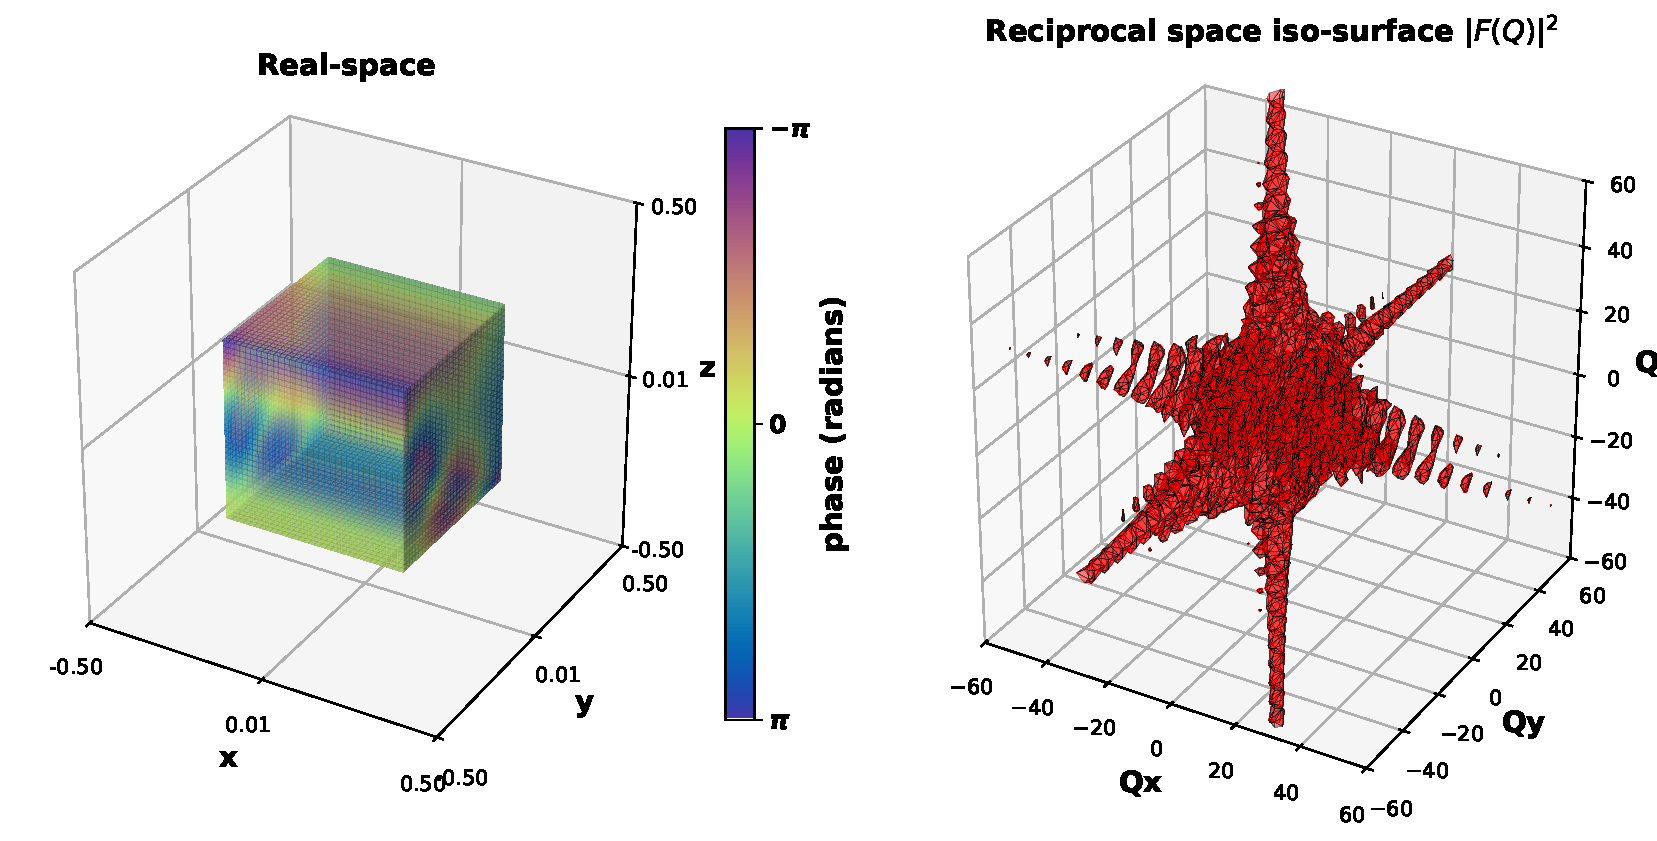
\includegraphics[width=\textwidth]{figures/Intro/cube_hihgstrain.pdf}
    \caption{Illustration of the squared modulus of the Fourier transform of a cube with an applied displacement field. 
    The phase derived from the projection of the displacement on the scattering vector is represented in on the left. On the 
    right the corresponding diffraction pattern. It is visible the deformation of the Bragg peak with respect to the 
    one in Fig.\ref{fig:cube} for the perfect lattice case. }
    \label{fig:cube_strain}
\end{figure}

From Eqs.\ref{eq:strain_fin4}–\ref{eq:fourie_relation} we can intuitively imagine that the distortion of the diffraction 
pattern is linked to (i) the \textit{magnitude} of the displacements, (ii) the \textit{number} of lattice sites involved, 
(iii) the \textit{coherence} of each local contribution $S(\mathbf{R}_i)e^{i\phi(\mathbf{R}_i)}$ with respect to its 
neighbors. The interplay of these parameters gives rise to many possible distortions of the ideal crystal diffraction.

Lattice sites that are displaced with respect to the perfect lattice scatter at slightly different Bragg angles. This 
produces intensity shifted to different $\mathbf{q}$ values around the Bragg peak. The displacements are 
proportional to the complex phases in the kinematic sum. If the phases are the same 
across many sites, the sum is coherent, and the resulting diffraction signal remains localized and peaked. On the 
other hand, if the phases vary from site to site, coherence is lost, and the diffraction pattern becomes more irregular.

It follows that the more voxels are involved in incoherent phase variations, the more speckled the diffraction pattern 
becomes, since each contribution departs differently from the original Bragg condition. This is often called \textit{heterogeneous} 
strain. Conversely, in the case of equal displacements across many sites, the contributions remain coherent, leading to 
the so-called \textit{homogeneous} strain. The diffraction signal in this case tends to split into two peaks: one 
corresponding to the pristine lattice and one to the uniformly strained lattice.

An important case, discussed later in the text, is the high-strain regime, in which a significant fraction of lattice 
sites undergo large heterogeneous displacements. This should be contrasted with localized defects such as dislocations 
or grain boundaries (not treated here), where relatively large displacements are confined to only a few lattice sites.

\subsection{Noise}

We should now introduce the last ingredient to our derivation, the presence of noise. 
When dealing with real life experiment we have to consider that photons are quantum particles, thus their arrivals on 
the detector surface are random independent events. Here, because of the discrete nature of photons, a statistical approach 
based on the average arrival rate is required. It follows that an uncertainty is intrinsically associated to the estimate, 
hence the emergence of a source of noise. The statistical model describing these phenomena is known as Poisson 
statistic \cite{Poisson}. In particular, given a constant \textit{average} rate of arrival $\eta$ over a unit 
of time, the \textit{expected} number of photons after an exposure time $\tau$ is $\mu = \eta \tau$, and the probability 
of detecting $N$ photons over an observing time $\tau$ is given by the formula: 

\begin{equation}
    p(N) =  \frac{(\eta \tau)^N e^{-\eta \tau}}{N!}
    \label{eq:poisson}
\end{equation}

also called \textit{Poisson probability distribution}. It can be proven that for the Poisson distribution 
the variance equals the mean $\mu = \sigma^2 = \eta \tau $. Moreover, we can intuitively think the expected number of photons 
collected during a time $\tau$ by a pixel in position $\mathbf{q}_i$ to be proportional to the intensity in \ref{eq:fourie_relation}
evaluated in $\mathbf{q}_i$ and integrated over a time $\tau$.
At this point, if we were to make a measurement, in absence of background, we would have at position $\mathbf{q}_i$ an 
expected integrated intensity $\mu = \bar{I}(\mathbf{q}_i)$ with an uncertainty of $ \sigma = \sqrt{\bar{I}(\mathbf{q}_i)}$. 
Being the Signal-to-Noise-Ratio (SNR) defined as $SNR = \mu / \sigma$ we obtain in our case: 

\begin{equation}
    SNR =  \frac{1}{\sqrt{\bar{I}(\mathbf{q}_i)}} 
    \label{eq:SNR}
\end{equation}

Though very simple, this equation is important and deserves some comments.
First, we can observe that in the limit of infinitely long integration times or infinite intensity (infinite flux), 
the $SNR \rightarrow 1$, meaning that we would in principle able to deterministically measure the diffraction pattern, 
in this case noiseless. Secondly, being most of the intensity of a diffraction 
pattern concentrated in the center of the Bragg peak, (Fig.\ref{fig:square_ft}) we can deduce from Eq.\ref{eq:SNR} that Poisson 
noise is affecting regions at high $\mathbf{q}$ much more than at the center. During PR, this uncertainty in high $\mathbf{q}$ ranges 
reflects, in real space, to a lower accuracy on fine resolution features of the reconstructed objects. The SNR, by mostly 
affecting lower photon counts regions, typically located at high $\mathbf{q}$ values, sets a limit to the actual
attainable direct-space resolution.

% This uncertainty originated by the noise becomes crucial in case of high-strain. In fact, we have seen that displaced 
% lattice sites scatter at different $\mathbf{q}$, far from the Bragg peak. Moreover, the amount of this deviated signal 
% is proportional, for Parseval theorem, to the amount of lattice sites (or voxels when DFT are used) responsible for that 
% contribution. If this number is small and the heterogeneous strain is high the signal is weak and far from other 
% contributions, and therefore can be buried in noise. It follows that during the reconstructions, the amplitude of those 
% voxels of the object is not fully retrieved, hence the presence of dips in the electronic density or holes.  

% Intuitively we can imagine that the amount of distortion affecting the diffraction pattern is linked to the \textit{magnitude} of 
% the displacements and to the \textit{number} of lattice sites altered by the displacement. However, considering the object made of voxels, 
% more important to the final diffracted intensity is the coherence of each $s_j e^{i \phi_j}$ with respect to the neighbors. 
% An important case that will be discussed 
% later in the text is the \textit{high-strain case} in which a significant amount of lattice sites are affected by large displacements. 
% Other cases of defects, dislocations, grain boundaries (not treated here) are often localized in few lattice sites where in turn 
% the displacement can be relatively large. 


\section{BCDI at ESRF - ID01}\label{chp:id01}

We have so far discussed the theoretical foundations for the understanding of the BCDI technique. It is now time to 
see the practical aspects. \\
Starting from the source of the probing radiation downstream to the detectors we will focus on the most important stages, 
necessary to envision the experimental conditions as well as typical numbers (resolution, energies, sizes).

BCDI experiments require a \textit{coherent} X-ray beam focussed on a volume of few cubic microns. Moreover, such beam also needs 
to deliver a sufficient amount of photons to the sample which, being in the micrometer range as well possesses a limited scattering 
power. Such properties today can only be achieved in large scale facilities like synchrotrons and free electron lasers (FELs). \\
We know that electromagnetic waves can be generated by accelerating charges \cite{griffiths}. In synchrotron facilities 
electrons travel in a large circular ring (\textit{storage ring}) at relativistic speeds and X-rays are produced deflecting their trajectories 
with the help of magnets. Depending on the magnet size, magnetic field and spatial configuration the X-ray beam is generated 
with different properties. Typically, these configurations are grouped into two main categories, namely: \textit{bending magnets} 
and the more modern Insertion Devices (ID) like \textit{wigglers} and \textit{undulators}. In synthesis, while bending magnets 
produce X-rays in a broad energy spectrum with relatively low intensity, wigglers exploit series of smaller magnetic dipoles 
to increase the intensity of the radiation. Undulators on the contrary leverage the periodicity of the dipoles to stimulate 
coherent emission, hence sharpening the energy bandwidth around tunable peaks and increasing the intensity as well. 
The radiation generated by the latter is the most suited for coherent diffraction experiments because of its inherent 
higher coherence.
An illustrative explanation is provided by Fig. \ref{fig:synchrotron} while an exhaustive description of synchrotron radiation can be found 
in the notable book from Prof. Giorgio Margaritondo \cite{margaritondo}.\\
The X-rays produced in these sections travel along straight lines, tangential to the storage ring, where they go through 
a number of optical elements dedicated to the spatial and spectral filtering as well as focusing and collimation, down 
to the experimental hutch where they finally radiate the samples. These are called \textit{beamlines}, and they are usually 
designed and equipped for a specific class of techniques. 

At the European Synchrotron Radiation Facility (ESRF) the ID01 beamline was conceived to combine the lattice parameter 
resolution provided by X-ray diffraction with spatial resolution of imaging techniques \cite{leake_nanodiffraction_2019} and 
is able to offer various techniques for the investigation of strain at nanoscale, including BCDI. 

\begin{figure}[H]
    \centering
    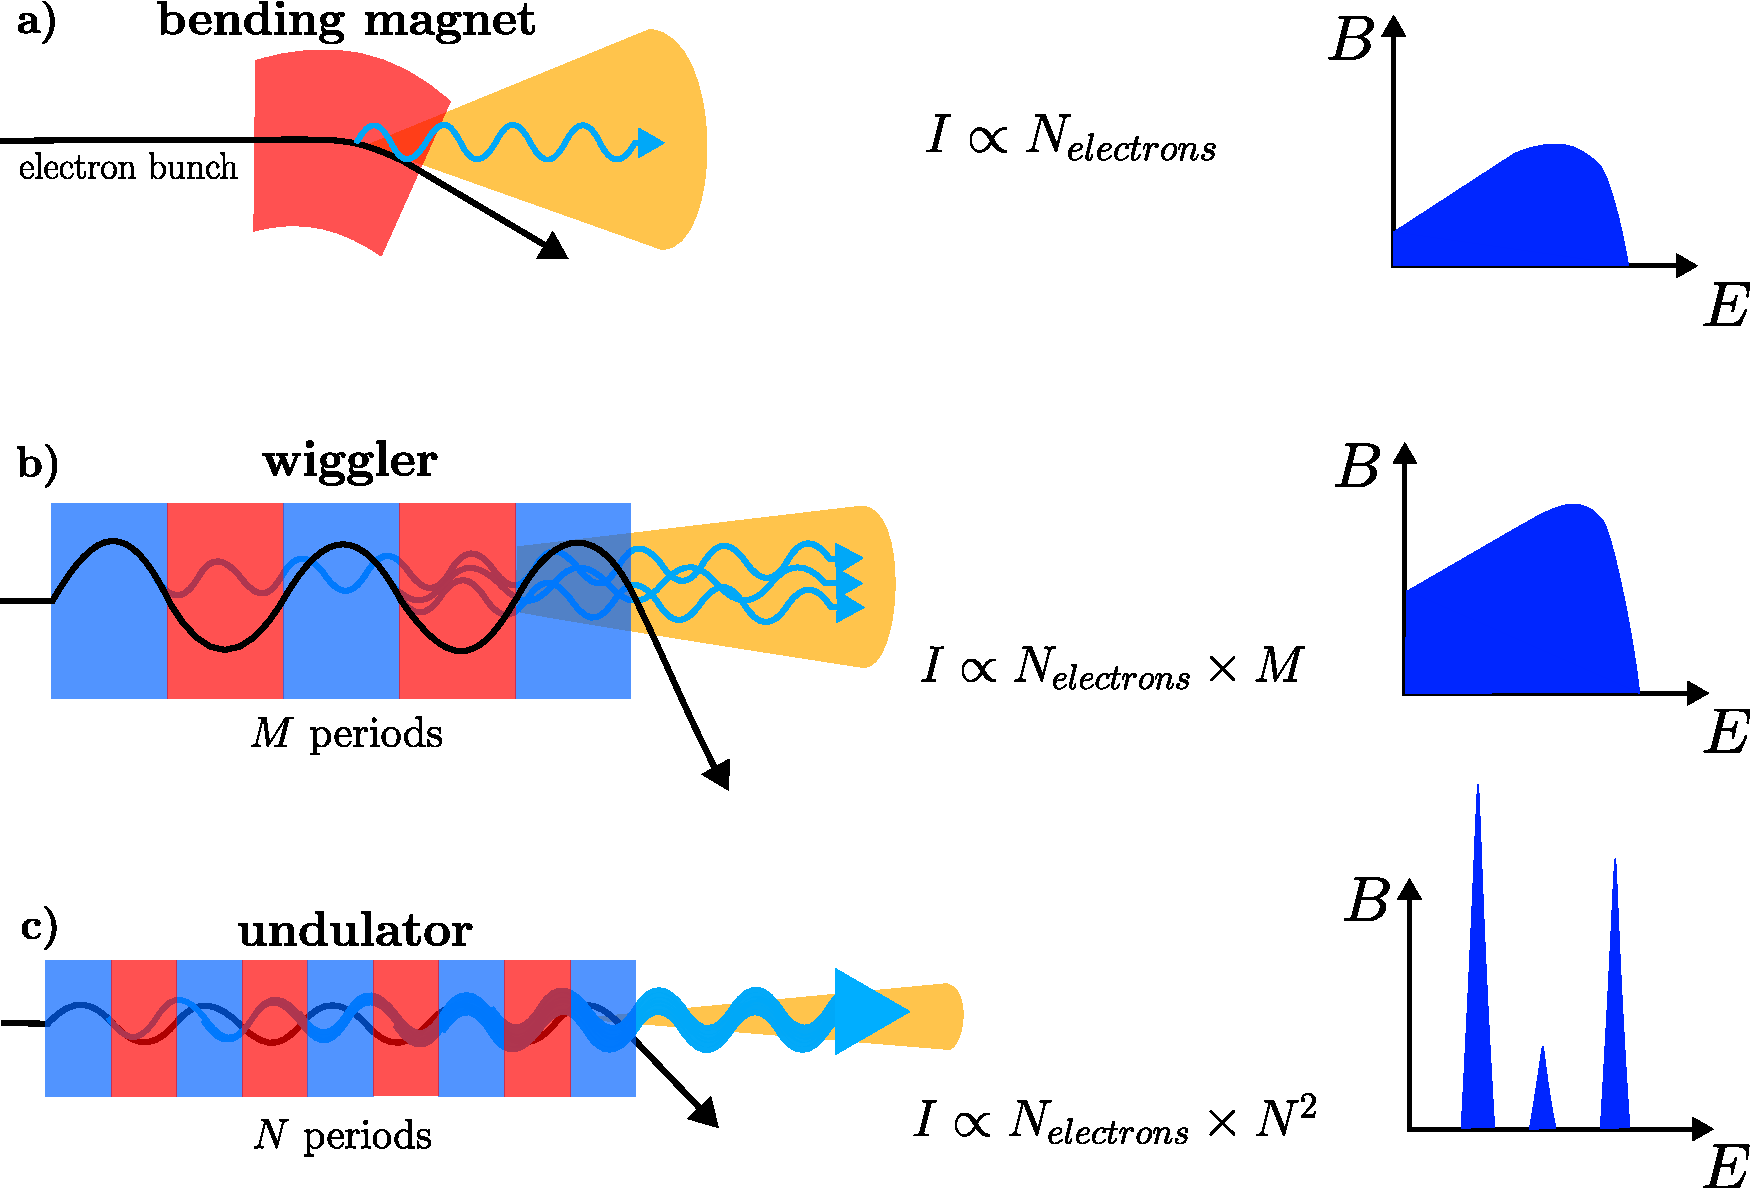
\includegraphics[width=\textwidth]{figures/Intro/synchrotron.pdf}
    \caption{\textbf{Illustration of the three main synchrotron X-ray sources.} \textbf{a)} The intensity of the 
    bending magnet radiation scales with the number of electrons being deflected. The beam is emitted with a broad 
    horizontal divergence and the spectrum covers multiple wavelengths. \textbf{b)} The wiggler exploits a series of 
    magnets to increase the intensity of the emitted radiation. \textbf{c)} In the undulator the periodicity of the poles 
    is such that the photons are emitted with higher temporal coherence. The X-ray beam shows narrower emission cone (increased 
    transversal coherence) as well as higher intensity and narrower bandwidths.}
    \label{fig:synchrotron}
\end{figure}

\subsection{Beam size}

Typical BCDI experiments are focused on single nanoparticles. The diffraction pattern is the result of the scattering of 
a single crystal in Bragg condition. It is therefore necessary to have a beam size of the order of the size of the crystal. 
At ID01 the beam size can scale down to $35 \times 35 nm$ \cite{esrf_id01}, but typical sizes are around $ 1 \mu m^2$. 
A too large beam could shine some neighbor particles which, if in Bragg condition, could contaminate the diffraction pattern. 
These often appear as isolated bright spots, called \textit{aliens} \cite{Pelzer:te5062}. On the contrary, regions of the same particle that 
are not illuminated do not contribute to the diffraction pattern, therefore are not imaged in the reconstructed objects. 

\begin{figure}[H]
    \centering
    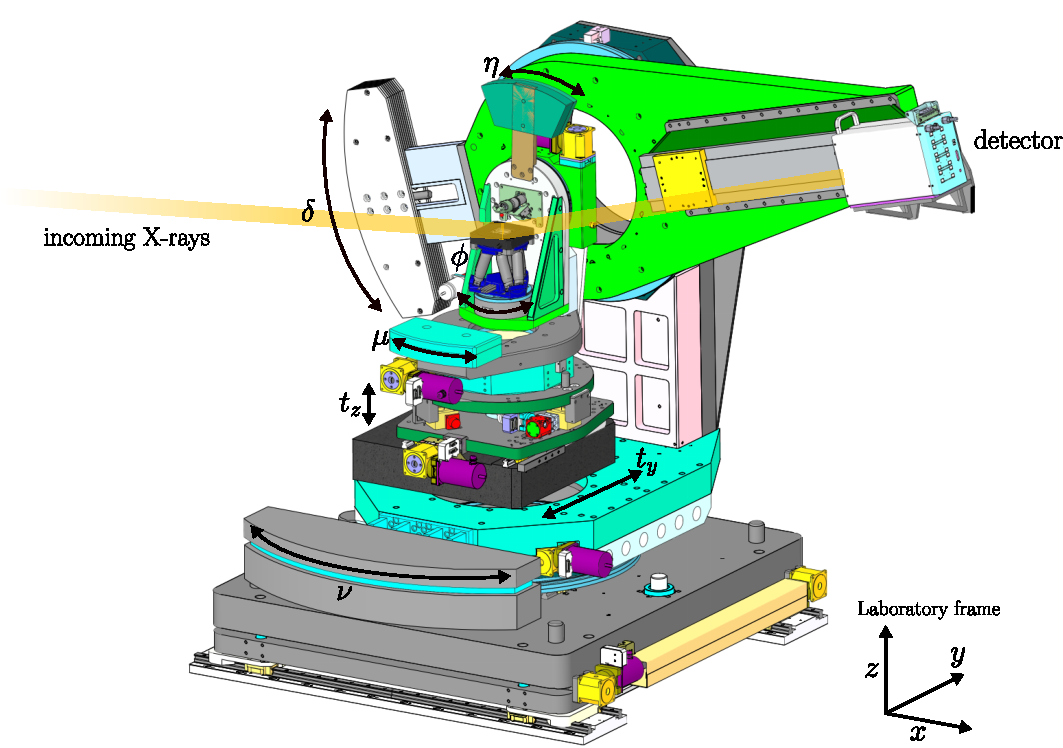
\includegraphics[width=\textwidth]{figures/Intro/beamline.pdf}
    \caption{Computer Aided Design of the diffractometer at the ID01 beamline with the corresponding degrees of freedom. 
    Adapted from \cite{Atlan2023}}
    \label{fig:diffractometer}
\end{figure}

\subsection{Energy and flux}
An important figure of merit for the characterization of synchrotron radiation is \textit{brilliance}. It measures 
the number of photons populating the beam per unit of time, area and solid angle within a 0.1 $\%$ fraction of bandwidth relative 
to a certain energy. 
It is therefore defined as:

\begin{equation}
    B = \frac{\text{nb photons}}{dt \cdot dA \cdot d\Omega \cdot 0.1\% dE/E} 
\end{equation} 
 
ID01's radiation is generated by up to three undulators, one of which is tuned to deliver the optimum brilliance 
in the range of 6 - 11.5 keV. This energy range is particularly suited for coherent diffraction experiments on crystals . 
In fact, at lower energy absorption effects from optical elements and air start being important, hence reducing the net 
flux available on the sample. On the other hand, at higher energies other problems arise, namely: (i) the degree of  
coherence drops significantly (see next paragraph) and (ii) the diffraction patterns, for fixed detector distance, shrink 
in a lower number of pixels causing problems for PR. \footnote[1]{ 
This is related to the concept of the \textit{oversampling condition} discussed in the next chapter}

\subsection{Coherence}

This fundamental property of electromagnetic radiations is probably the most important for CDI. In the derivation of the 
scattering equation Eq.\ref{eq:scattering_pointlike} and following, we have always assumed the incident radiation to be 
described by a plane wave, perfectly monochromatic ($\Delta \lambda \neq 0 $) and with no angular spreading ($\Delta \mathbf{k} = 0$). 
In the ideal case, the wave-field is perfectly coherent, meaning that the relative phase between any two points in space is 
completely well-defined.
In reality, electromagnetic waves have finite temporal duration and therefore, by Fourier transform relations, a finite 
spectral bandwidth. Likewise, they are produced by extended sources and observed at finite distances, which implies a 
finite angular spread of the wave-vectors.
These limitations introduce phase decorrelation between fields evaluated at two different points, either \textit{along} the propagation 
direction (due to bandwidth) or \textit{across} it (due to angular dispersion).
For this reason, it is useful to introduce quantities that characterize the ``degree of coherence'' of the radiation. 
An intuitive approach is to define a \textit{longitudinal coherence length}, associated with phase delays from spectral 
bandwidth, and a \textit{transverse coherence length}, associated with phase delays from angular spread. \\

\textbf{Longitudinal Coherence Length} $L_l$: is defined as the distance after which two beams originated in the same point and 
characterized by a wavelength difference $\Delta \lambda = 0 $ have a phase difference of $\pi$, being therefore in phase opposition. 
This means that after a distance $2L_l$ the two waves are back in phase. If the first wave of wavelength $\lambda$ needs 
$N$ cycles to cover $2L_l$ it follows that the second wave with wavelength $\lambda + \Delta \lambda$ will need $N-1$ cycles. 
Therefore: 
\begin{equation}
    \begin{aligned}
    N\lambda = (N-1)(\lambda + \Delta \lambda) \\
    \text{thus, } \Delta \lambda(N-1) = \lambda 
    \end{aligned}
\end{equation}

In case of small $\Delta \lambda / \lambda $ we can approximate $N-1 \approx N$, and obtain $N \approx \lambda / \Delta \lambda$. 
This leads us to the expression for the longitudinal coherence length: 

\begin{equation}
    L_l \approx \frac{\lambda^2}{2\Delta \lambda}
\end{equation}

As expected the longitudinal coherence increases with the monochromaticity of the beam. On the contrary it significantly 
worsens for high energies, as anticipated above. 

\textbf{Transversal Coherence Length} $L_t$ is defined as the distance between two points $A$ and $B$ sitting on a plane at distance $D$ from a 
source of size $ S$ for which both $A$ and $B$ are out of phase. Fig. shows geometrically that this distance, 
when $S \ll D \rightarrow \theta \approx 0 \rightarrow \cos(\theta)\approx 1$, the transversal coherence length is given by: 

\begin{equation}
    L_t \approx \frac{\lambda D}{2 S}
\end{equation}

\begin{figure}[H]
    \centering
    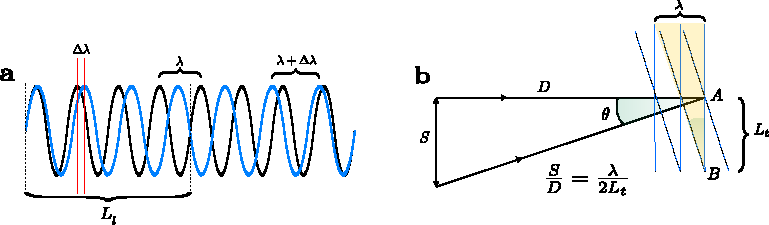
\includegraphics[width=\textwidth]{figures/Intro/coherence.pdf}
    \caption{\textbf{a} Sketch of the longitudinal coherence length $L_l$. Two plane waves with slightly different wavelength 
    originating in phase are out of phase after propagating over a distance equal to $L_l$. \textbf{b} Sketch of the 
    transverse coherence length $L_t$. Two plane waves emitted at slightly different angles from an extended source 
    are evaluated on a distant plane. They become out of phase when separated by $L_t$. 
    Being the highlighted triangle similar to the bigger one in black, an expression for $L_t$ can be derived from 
    simple geometrical considerations}
    \label{fig:coherence}
\end{figure}

Also in this case we see the coherence decreasing for high energies.
Moreover, the dependence on $S$ and $D$ explains the challenges to build long beamlines (118 meters for ID01) and
reduce the electron bunches in storage rings. The transverse coherence length can be easily lifted to a coherence surface 
for a source extended in 2D ($L_t^{hor} \times L_t^{ver}$).\\

Given these premises we can now calculate the coherence \textit{volume} ($L_l \times L_t^{hor} \times L_t^{ver}$) available 
ID01 for a typical X-ray energy used in BCDI. Given the source sizes of $60 \mu m$ horizontally and $15 \mu m $ vertically, 
at 8 keV ($\lambda = 1.55$ \r{A}) we obtain a transverse coherent surface of $152 \mu m \times 610 \mu m$. The longitudinal
coherence length is found to be approximately $0.8 \mu m$ considering the $\Delta \lambda / \lambda \sim 10^{-4}$ typical of the 
double Si (111) crystal monochromator. It follows that often, in BCDI experiments, the limitation on the particle size is 
given by the longitudinal coherence \cite{Steven2009}. \\ 

The coherence volume specifies the maximum spatial separation between two scatterers for which their scattered waves 
remain mutually coherent and can interfere. For this reason, while classical X-ray diffraction is limited to the interference 
of few lattice points, in the order of few \r{A}, the X-ray beam at ID01 can enable interference from objects separated by the order of few 
$\mu m$. In BCDI, the sample size is usually smaller than the coherence volume, meaning that scattering from all parts 
of the crystal, even from opposite surfaces, remains mutually coherent. This results in the characteristic interference 
pattern observed.

\subsection{Ewald sphere and Rocking curves}

At this point of the dissertation we should address the procedure related to data acquisition. In particular, in order to 
understand the generation of 3D diffraction patterns from the 2D images collected by the detector we need to introduce the 
concept of Ewald sphere. 


We have said that in BCDI we focus on a single $hkl$ node of the reciprocal lattice, and we collect the diffraction pattern 
of the full diffracting crystal around that Bragg peak. Given the exit wave-vector $\mathbf{k}$ 
pointing at the Bragg peak, we could draw a sphere of radius $k$ centered in the sample and find the diffraction pattern 
of interest at the intersection of such sphere with the reciprocal lattice in the $hkl$ node.  Such sphere is called 
\textit{Ewald sphere} and it is illustrated in Fig.\ref{fig:ewald}. More generally, one can state that the diffraction 
from a wave-vector $\mathbf{k}$ occurs only in those reciprocal lattice points that intersect the Ewald sphere
of radius $k$. \\
Moreover, the surface of the sphere around the Bragg peak tells us the signal captured by the 2D detector. 
In order to collect the 3D pattern one usually needs to apply a small rotation the sample along the axis that crosses the sample horizontal and 
perpendicular to $\mathbf{k}$ such that the Bragg condition is found for the same $hkl$ node in a slightly shifted position in space. 
The Ewald sphere is no longer cutting the diffraction pattern in the precise $hkl$ node but in the extended peak broadened by the 
finite size effect. When this rotation, called \textit{rocking curve}, is performed along both directions from one extremity of 
the pattern to the opposite, a 2D image is recorded by the detector at each angular step. The full stack of 2D images creates 
the full 3D diffraction pattern. 

\begin{figure}[H]
    \centering
    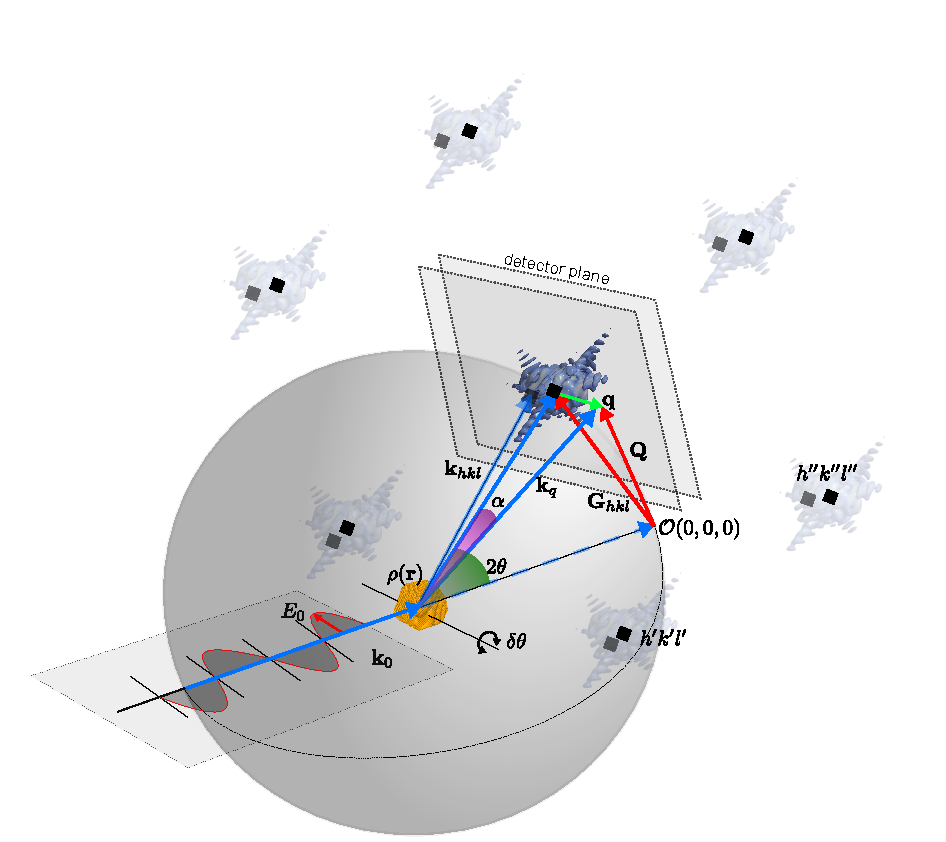
\includegraphics[width=\textwidth]{figures/Intro/ewald1.pdf}
    \caption{Illustration of the typical geometry for a BCDI experiment and the Ewald sphere (not in scale). A monochromatic plane wave approximates a 
    coherent X-ray beam that fully illuminates sample with a wave-vector $\mathbf{k_i}$. A diffraction pattern given by Eq. 
    \ref{eq:strain_fin4} is formed around each $hkl$ node. Of the different reciprocal lattice nodes a single one is 
    selected for the measurement. The Ewald sphere, of radius $\mathbf{k}_{hkl}$ shows that the diffraction condition is met
    at the intersection with the $hkl$ node. The detector plane, perpendicular to the $\mathbf{k}_{hkl}$ vector, captures 
    a swathe of Ewald sphere extending of an amount $\mathbf{q} = \mathbf{k}_{q} - \mathbf{k}_{hkl}$ around the $hkl$ node.
    Different slices of the diffraction pattern are acquired rotating the sample at each angle  $2\theta \pm N\delta \theta$. 
    Notice that this angle is equivalent to the $\eta$ angle in Fig.\ref{fig:diffractometer}, typically tuned during the 
    rocking curve.}
    \label{fig:ewald}
\end{figure}

This approach assumes that the surface of the Ewald sphere in the vicinity of the Bragg peak can be approximated to be flat. 
In reality onto the detector is projected the slice of diffraction pattern extending over a swathe of Ewald sphere of 
radius $r = k$. It follows that for higher energies this approximation holds better as the contact angle is decreasing. 
Additionally, another consequence of the reduction of the contact angle at high energies is that the reciprocal space 
is shrinking. In order to understand this can consider that:
geometrically the contact angle is equivalent to the angle $\alpha$ between the vectors $\mathbf{k}_\mathbf{q}$ and $\mathbf{k}_\mathbf{hkl}$. 
Being now $\delta q = |\mathbf{k}_\mathbf{q} - \mathbf{k}_\mathbf{hkl}| = |\mathbf{k}_\mathbf{q}|\sin (\alpha)$ one 
could infer that for higher energies (larger $\mathbf{k}_\mathbf{hkl})$ the portion of diffraction pattern 
explored by $\delta q = |\mathbf{k}_\mathbf{q}|\sin (\alpha) \approx |\mathbf{k}_\mathbf{q}|\alpha$ 
is now shrunk into a smaller $\alpha$. This effect compresses the whole reciprocal lattice and thus the  
diffraction pattern as well, around the $hkl$ node. This issue causes constraints in the sampling as will be discussed 
in the next Chapter.

% This approximation holds depending on the distance between the sample and the detector. One could in fact calculate 
% the width of the angle separating the detector plane and the swathe of Ewald sphere projected onto it. Given a detector 
% with a sensing area of $512 \times 512$ pixels of $55x55 \mu m^2$ area

% \subsection{Detectors}

